\chapter{A Foundation for Streams}
\label{cha:foundation}
\headerblock{
  \headerquote{Almost every problem that you come across is befuddled with all kinds of extraneous data of one sort or another; and if you can bring this problem down into the main issues, you can see more clearly what you’re trying to do.}{Claude Shannon}

  \headerhide{
    \headerbreak{}

    \headerimage{img/xkcd-standards.png}
  }
}

This section lays the groundwork for the rest of the technical content of this dissertation: we present our core type system for distributed streams. This is based on \emph{synchronization schemas}~\citeMain{pods21}, which evolved from earlier work on \emph{data-trace types}~\citeMain{festschrift18,pldi19}.
Our stream types are an abstraction over Mazurkiewicz traces, studied in concurrency theory to model distributed sets of events~\cite{mazurkiewicz1986trace,DiekertR1995}.

A stream type $S$ describes the structure of events in the stream;
semantically it will denote a collection of partially ordered traces.
Formally, there are multiple ways to encode and view partially ordered traces.
First, the global view as a strutured batch $\batchtype{b}{S}$.
This is a parsed structure: for example, if $S$ is composed of two stream types in parallel, $S_1$ and $S_2$, then a batch of type $S$ is a pair of a stream of $S_1$ and a stream of $S_2$.
Second, there is a more local view of elements of the stream.
$S$ gives rise to a type for events $\eventtype{e}{S}$,
which are possible individual elements in the stream.
Then, a sequence of events is a linearization of the stream,
or a partially ordered set labeled with events is a partially ordered trace
for the stream.

\section{Stream Types}

\begin{definition}
Let $T$ denote a base type in the following grammar.
A \emph{stream type} is a type defined syntactically by the following grammar:
\[
  S \quad ::= \quad
    \hier{T}{S} \mid
    \parcomp{S}{S} \mid
    \keyby{T}{S} \mid
    \relleaf{T} \mid
    \empstream{}
\]
\end{definition}

We also have the following abbreviation for a sequence of \texttt{T}:
\[
  \seqleaf{T} := \hier{T}{\empstream{}}.
\]

\section{Views of Streams}

\subsection{Streams as Structured Batches}

The following syntax defines concrete \emph{structured} stream instances for each of the
stream types, which we call \emph{batches} because they represent data
collected into a static bundle.\footnote{Thanks to Joe Cutler for this suggestion.}
To define a concrete stream instance, one either defines a pair, a sequence, or a bag (unordered multiset).
\[
  B \quad ::= \quad
    (B, B) \mid
    [B, B, \ldots, B] \mid
    \{B, B, \ldots, B\} \mid
    t: T
\]

Batches are typed using the following typing rules:

\begin{mathpar}
    \inference[Synch]
    {
      t_i: T \\
      \batchtype{b_i}{S}
    }
    {
      \batchtype{[b_0, t_1, b_1, t_2, b_2, \ldots, t_m, b_m]}{\hier{T}{S}}
    }
    \\

    \inference[Par]
    {
      \batchtype{b_1}{S_1} \\
      \batchtype{b_2}{S_2} \\
    }
    {
      \batchtype{(b_1, b_2)}{\parcomp{S_1}{S_2}}
    }

    \\

    \inference[ParBy]
    {
      k_i: K \\
      k_i \ne k_j \text{ for } i \ne j \\
      \batchtype{b_i}{S} \emph{ nonempty}
    }
    {
      \batchtype{\{(k_1, b_1), (k_2, b_2), \ldots, (k_n, b_n)\}}{\keyby{K}{S}}
    }

    \\

    \inference[Bag]
    {
      t_i: T
    }
    {
      \batchtype{\{t_1, t_2, \ldots, t_n\}}{\relleaf{T}}
    }

    \inference[Emp]
    {
      \;
    }
    {
      \batchtype{[]}{\empstream{}}
    }
\end{mathpar}

The \emph{nonempty} requirement in the \textsc{ParBy} case is the inductive property that holds exactly when the batch has no occurences of $t: T$ for any base type $T$.
Specifically, $(b_1, b_2)$ is empty if $b_1$ and $b_2$ are empty;
a list is empty if and only if it is $[]$;
a bag is empty if and only if it is $\{\}$;
and $t: T$ is not empty.

\subsection{Stream Events and Dependence Relation}

A stream can also be thought of as a type for individual events in isolation.
Events can be either base types are tuples.
Tuples are needed because if $K_1, \ldots, K_n$ are types of keys and $T$ is a payload type,
an event is a tuple of an element of each key and an element of the payload.
Here is a grammar for events:
\[
  E \quad ::= \quad (E, E) \mid t: T
\]

We can also talk about events specific to a particular stream type:
$\eventtype{e}{S}$ means that $e$ is a valid event for a stream type $S$.
Notice that there are no rules for $\eventtype{t}{\empstream{}}$ -- there are no events of the empty stream type.

\begin{mathpar}
    \inference[Synch-1]
    {
      e: T
    }
    {
      \eventtype{e}{\hier{T}{S}}
    }

    \inference[Synch-2]
    {
      \eventtype{e}{S}
    }
    {
      \eventtype{e}{\hier{T}{S}}
    }
    \\

    \inference[Par-1]
    {
      \eventtype{e}{S_1}
    }
    {
      \eventtype{e}{\parcomp{S_1}{S_2}}
    }

    \inference[Par-2]
    {
      \eventtype{e}{S_2}
    }
    {
      \eventtype{e}{\parcomp{S_1}{S_2}}
    }

    \\

    \inference[ParBy]
    {
      k: K \\
      \eventtype{e}{S}
    }
    {
      \eventtype{(k, e)}{\keyby{K}{S}}
    }

    \inference[Bag]
    {
      e: T
    }
    {
      \eventtype{e}{\relleaf{T}}
    }
\end{mathpar}

However, a stream type is more than just its type of events.
In addition, a stream defines a \emph{dependence relation}: a symmetric binary relation
on pairs of events, which intuitively indicates whether one event synchronizes another.
The dependence relation written
$\deptype{e}{e'}{S}$ means that events $e$ and $e'$ are dependent
with respect to the stream tyep $S$ (the events should in particular satisfy $\eventtype{e, e'}{S}$).
This is defined by the following rules.
Notice that there are no rules for
$\empstream{}$ (because it has no events)
nor for $\relleaf{}$ (because all events in a bag are independent).

\begin{mathpar}
    \inference[Synch]
    {
      t: T \\
      \eventtype{e}{\hier{T}{S}}
    }
    {
      \deptype{e}{t}{\hier{T}{S}} \\
      \deptype{t}{e}{\hier{T}{S}}
    }

    \inference[Sub]
    {
      \deptype{e}{e'}{S}
    }
    {
      \deptype{e}{e'}{\hier{T}{S}}
    }
    \\

    \inference[Par-1]
    {
      \deptype{e}{e'}{S_1}
    }
    {
      \deptype{e}{e'}{\parcomp{S_1}{S_2}}
    }

    \inference[Par-2]
    {
      \deptype{e}{e'}{S_2}
    }
    {
      \deptype{e}{e'}{\parcomp{S_1}{S_2}}
    }
    \\

    \inference[ParBy]
    {
      k: K \\
      \deptype{e}{e'}{S}
    }
    {
      \deptype{(k, e)}{(k, e')}{\keyby{K}{S}}
    }
\end{mathpar}

Inductively, $\deptype{e}{e'}{S}$ is the smallest relation defined by the above rules.
If two events $\eventtype{e, e'}{S}$ are \emph{not} dependent, we say they are independent and write
$\indeptype{e}{e'}{S}$.
Dependence is constructive and decidable via the above rules, so we could have alternatively given a typing judgment for $\indeptype{e}{e'}{S}$.
For completeness, such a typing judgment is shown in \Cref{app:typing}.

We also could have given both $\deptype{e}{e'}{S}$ and $\indeptype{e}{e'}{S}$ as a single Boolean-valued function on pairs of events,
i.e. $\event{S} \times \event{S} \to \texttt{bool}$.

\subsection{Stream Linearizations and Equivalence Relation}

A \emph{linearization} is a sequence of events:
\[
  L \quad ::= \quad [E, E, \ldots, E]
\]
Notice that each event in the sequence may be different (they may even all have different types).
Linearizations support the operations of concatenation ($\cdot$), the interleaving relation
$\mathsf{inter}(l; l_1, l_2, \ldots)$,
and the element-wise product: for $t: E$ and $e_i: E$,
\[
  t \times [e_1, e_2, \ldots, e_n] := [(t, e_1), (t, e_2), \ldots, (t, e_n).
\]

Linearizations are typed using the following typing judgments:
\begin{mathpar}
    \inference[Synch]
    {
      t_i: T \\
      \lintype{l_i}{S} \\
      l = l_0 \cdot [t_1] \cdot l_1 \cdot [t_2] \cdots [t_m] \cdot l_m
    }
    {
      \lintype{l}{\hier{T}{S}}
    }

    \\

    \inference[ParBy]
    {
      k_i: T \\
      \lintype{l_i}{S} \\
      l_i \ne [] \\
      \mathsf{inter}(l; k_1 \times l_1, k_2 \times l_2, \ldots, k_n \times l_n)
    }
    {
      \lintype{l}{\keyby{T}{S}}
    }

    \\

    \inference[Par]
    {
      \mathsf{inter}(l; l_1, l_2) \\
      \lintype{l_1}{S_1} \\
      \lintype{l_2}{S_2} \\
    }
    {
      \lintype{l}{\parcomp{S_1}{S_2}}
    }

    \\

    \inference[Bag]
    {
      t_i: T
    }
    {
      \lintype{[t_1, t_2, \ldots, t_n]}{\relleaf{T}}
    }

    \inference[Emp]
    {
      \;
    }
    {
      \lintype{[]}{\empstream{}}
    }
\end{mathpar}

The dependence relation also gives rise to an equivalence relation on linearizations.
This equivalence relation is derived as follows:

\begin{mathpar}
    \inference[Indep]
    {
      \indeptype{e}{e'}{S}
    }
    {
      \equivtype{[e, e']}{[e', e]}{S}
    }

    \inference[Concat]
    {
      \equivtype{e_1}{e_1'}{S} \\
      \equivtype{e_2}{e_2'}{S}
    }
    {
      \equivtype{e_1 \cdot e_2}{e_1' \cdot e_2'}{S}
    }

    \\

    \inference[Refl]
    {
      \lintype{l}{S}
    }
    {
      \equivtype{l}{l}{S}
    }

    \inference[Trans]
    {
      \equivtype{e}{e'}{S} \\
      \equivtype{e'}{e''}{S}
    }
    {
      \equivtype{e}{e''}{S}
    }
\end{mathpar}

\subsection{Streams as Labeled Posets}

A \emph{partially ordered set} $(s, \le)$ is a set $s$ together with a binary relation $\le$ on pairs of elements of $s$ that is reflexive, transitive, and antisymmetric.

A \emph{labeled poset} (traditionally called a \emph{pomset}) of type $X$ is a
partially ordered set $(s, \le)$ together with a labeling function $\ell: s \to X$. We denote this $(s, \le, \ell)$. A labeled poset is different than a poset over $X$ because multiple elements may be labeled with the same element of $X$.
Two posets are \emph{equivalent} if the posets are isomorphic and the isomorphism exactly preserves the labeling $\ell$.

Then we can finally define the last view of streams, as partially ordered sets.
We write
\[
\posettype{(s, \le, \ell)}{S}
\]
if $\ell: s \to \event{S}$ such that the order is consistent with the dependence
relation in the following way:
\begin{enumerate}
\item[(i)] If $\deptype{\ell(i)}{\ell(j)}{S}$ then $i \le j$ or $j \le i$; and
\item[(ii)] No relaxation of $\le$ satisfies (i).
\end{enumerate}

\section{Examples}

% TODO

\section{Relation between Views}

\begin{proposition}
Linearizations are the same as sequences of events:
for any stream type $S$ and sequence $l = [e_1, e_2, \ldots, e_n]$,
\[
\lintype{l}{S} \quad \text{iff} \quad \eventtype{e_i}{S} \text{ for all } i.
\]
\end{proposition}

Given any stream type $S$, any linearization $\lintype{l}{S}$ gives rise to a labeled poset as follows:
if $l$ has length $n$, then we let $s = \{1, 2, \ldots, n\}$, and we define the labeling function $\ell(i) = l[i]$.
Then we define the ordering as follows:
$i \le j$ iff there is some sequence of indices
\[
i = i_0 < i_1 < \ldots < i_m = j
\]
such that each pair adjacent in the sequence is dependent:
\[
\deptype{l[i_0]}{l[i_1]}{S}, \deptype{l[i_1]}{l[i_2]}{S}, \ldots, \deptype{l[i_{m-1}]}{l[i_m]}{S}.
\]

This definition may look opaque, but captures the property that $l[i]$ and $l[j]$ are ordered: it is impossible to reorder them to get $l[j]$ before $l[i]$. The following proposition justifies this formally:
\begin{proposition}
Let $\lintype{l_1}{S}$ and $\lintype{l_2}{S}$ be two linearizations.
Then $\equivtype{l_1}{l_2}{S}$ if and only if the labeled posets for $l_1$
and $l_2$ are identical.
\end{proposition}

% TODO (bring content from sec5):
% - correspondence between linearizations and batches
%   - every linearization corresponds to a unique batch
%   - every batch can be linearized in at least one way (but maybe more)
% - empty stream (the batch corresponding to the empty linearization)

\section{Relation to Synchronization Schemas}
\label{45:ssec:illustrative-example}

\begin{figure}
    \centering
    \scalebox{0.8}{
    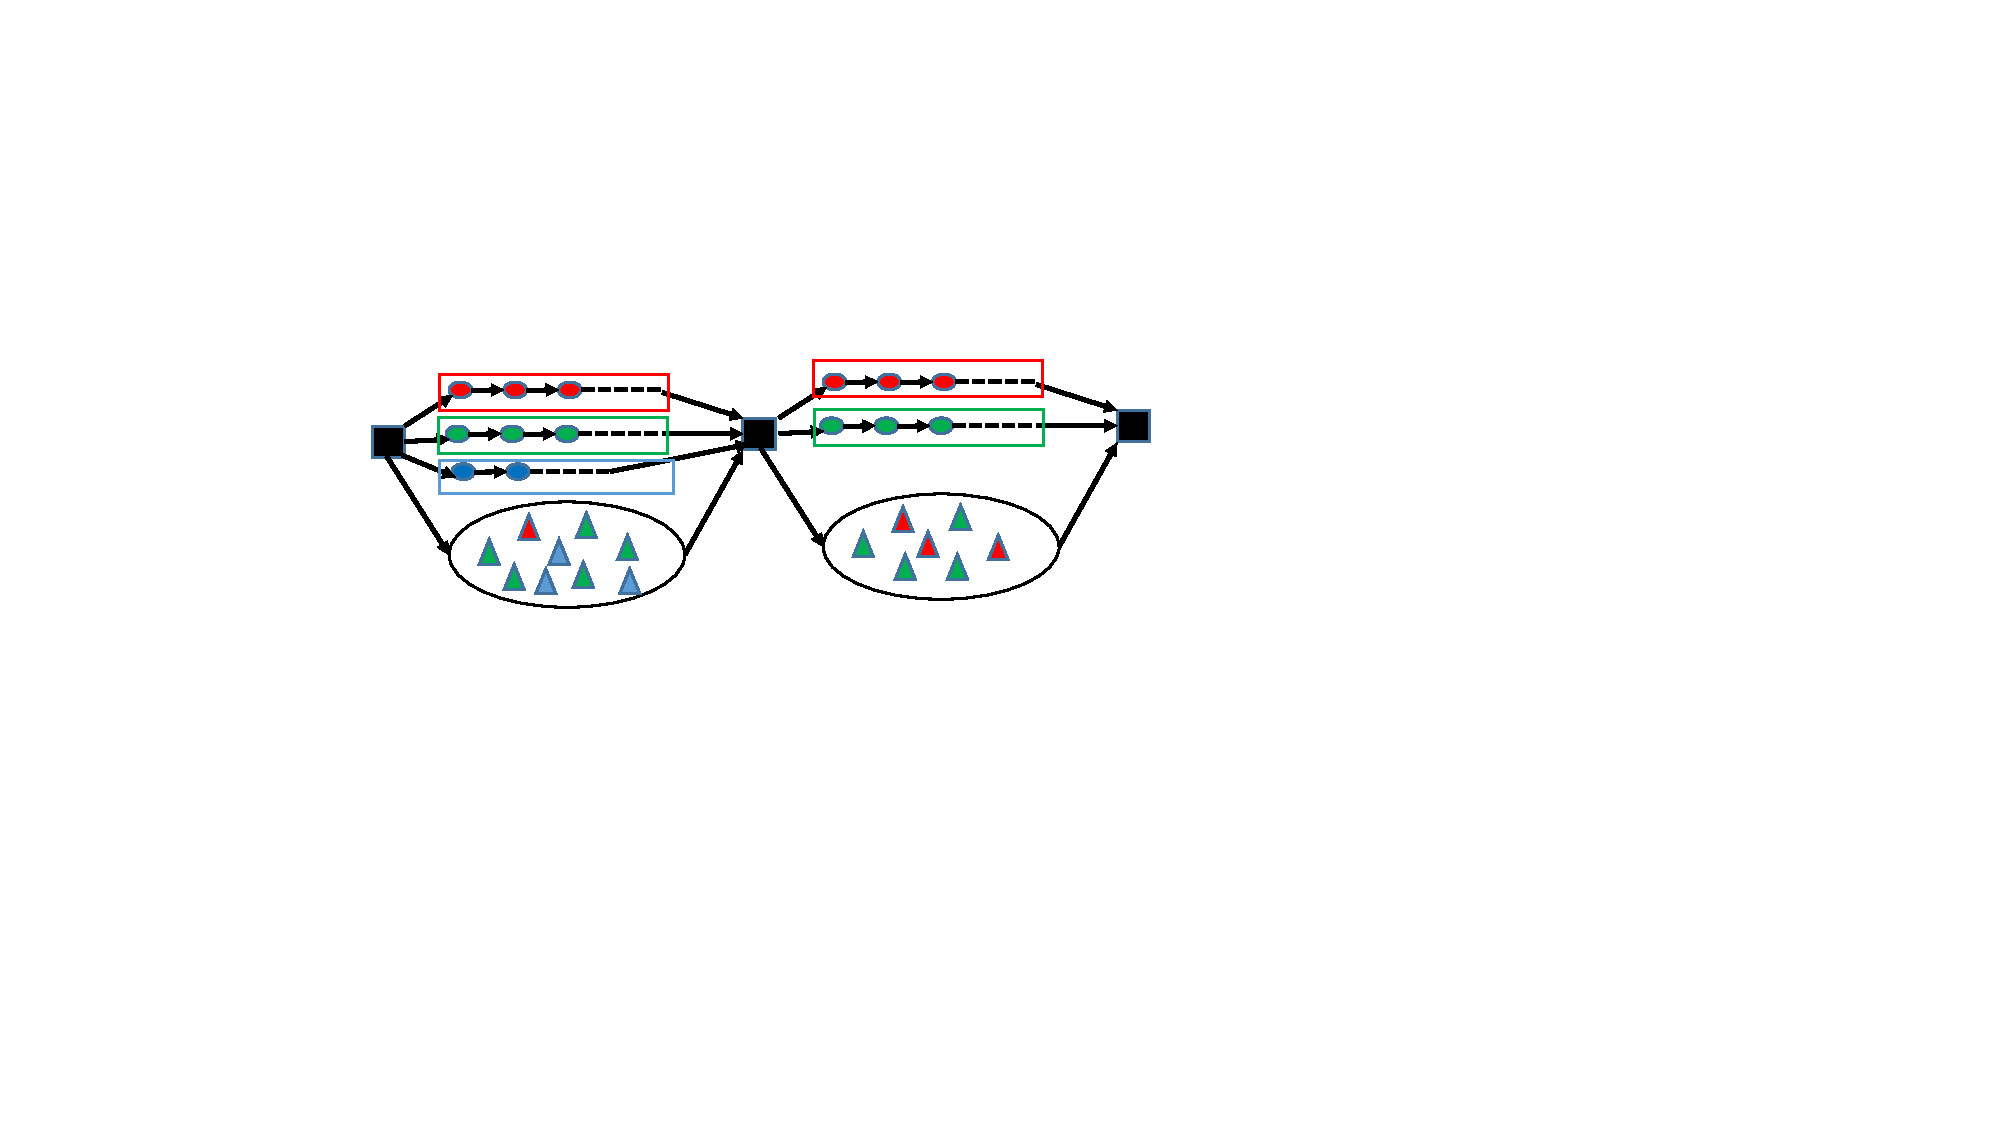
\includegraphics[width=3in]{figures/synchschemas/SPS2.pdf}
    }
    \caption{Illustrative partially ordered stream.}
    \label{45:fig:gps-sps}
\end{figure}

It is useful to understand how the stream types in this section relate to synchronization schemas.
We first need to define headers.
\begin{definition}[Headers and tuples]
A \emph{header} $H$
consists of a unique \emph{header name} \(\alpha\)
and \emph{fields} \(\hdrfield{\alpha_i}{\tau_i}\), for $1\le i\le n$,
where each \(\alpha_i\) is a \emph{field name}
and \(\tau_i\) is a \emph{field type}.
A \emph{tuple} $x$ of type \(H\), denoted $x : H$, is of the form
\(x = (x_1, x_2, \ldots, x_n)\), where each \(x_i : \tau_i\).
\end{definition}

When the context is clear, we identify each header \(H\) with its name \(\alpha\)
and likewise each field \(\hdrfield{\alpha_i}{\tau_i}\) with its name \(\alpha_i\).
We write \(\alpha_i \in H\) to mean that \(\alpha_i\) is a field of \(H\), and
\(x.\alpha_i\) to denote the value of \(x\) on \(\alpha_i\).
For a set $\mathcal{H}$ of headers, we write
$x: \mathcal{H}$ if $x : H$ for some $H \in \mathcal{H}$.
% and $\tup(\mathcal{H})$ for the set of all $x: \mathcal{H}$.

\begin{definition}[Synchronization Schema]
A \emph{synchronization schema} is a stream type $S$
where the base types $T$ present in $S$ are sets of headers.
\end{definition}

\begin{example}
\label{45:ex:taxi-distance-schema-headers}
Consider a stream of taxi events, where each is a GPS measurement, an indication of a taxi ride begin or a ride end, or an end-of-hour synchronization marker.
GPS data for each taxi is described by the header \texttt{GPS(location: pos, taxiID: int)}, where \texttt{pos} indicates the type of a GPS measurement---three dimensional coordinates, for instance.
Completed ride data is described by the header \texttt{RideCompleted(rideID: int, taxiID: int, passengerID: int, cost: int)}.
Finally, end-of-hour events are used to synchronize in time; these are described by the header \texttt{EndOfHour(date: date, hour: int)}.
\end{example}

The base rule $\relleaf{\mathcal{H}}$  defines a stream corresponding to a bag of $\mathcal{H}$-events, that is, events labeled with tuples of type $\mathcal{H}$. To combine the base rule (leafs) in complex schemas we use the other three rules. \hier{\mathcal{H}}{S} defines a parent relation between $\mathcal{H}$-events
and $S$-events---events labeled with any of the headers appearing in the schema $S$, and denotes a stream consisting of a sequence of $\mathcal{H}$-events that act as synchronization markers, interspersed with sub-streams of type $S$.
\keyby{K}{S} partitions a schema $S$ based on a set of key fields $K$,
and denotes a set of streams of type $S$, indexed by the values for the keys in $K$.
Finally, $\parcomp{S_1}{S_2}$ describes a sibling relation between schemas $S_1$ and $S_2$,  and corresponds to a parallel composition
of streams of types $S_1$ and $S_2$.

We use the following notational abbreviations.
When a set of headers consists of a single header $H$, we write $H$ instead of $\{H\}$.
We use $\seqleaf{\mathcal{H}}$ for
$\hier{\mathcal{H}}{\relleaf{\varnothing}}$,
 where $\varnothing$ is the empty set of headers, and such a schema corresponds to a totally ordered sequence of $\mathcal{H}$-events.
Finally, we write $\parthree{\ss_1}{\ss_2}{\ss_3}$
for the parallel composition of three schemas, which is short for
$\parcomp{\parcomp{\ss_1}{\ss_2}}{\ss_3}$ (note that parallel composition is associative).

\begin{example}
\label{45:ex:taxi-distance-schema}
We can define the schema for the input of the example in  \Cref{45:ex:taxi-distance-schema-headers} in a bottom up fashion in the following manner.
First, $S_1 = \keyby{\texttt{taxiID}}{\seqleaf{\texttt{GPS}}}$ denotes that \texttt{GPS} events are partitioned by the key \texttt{taxiID} and  are totally ordered for each taxi.
Second, $S_2 = \relleaf{\texttt{RideCompleted}}$ denotes that \texttt{RideCompleted} events are unordered, and can be considered to be a bag.
Finally, $S = \hier{\texttt{EndOfHour}}{\parcomp{S_1}{S_2}}$ denotes that \texttt{EndOfHour} events synchronize the events in $S_1$ and $S_2$, each of which can be processed in parallel as they are independent.
It is often helpful to visualize schemas as forests. \Cref{45:fig:example-schema} illustrates the schema for the example.
Siblings correspond to the \parcomp{S_1}{S_2} constructor while the rectangular box,
labeled with the key fields, corresponds to the \keyby{K}{S} constructor.
A parent node with several children corresponds to the $\hier{\mathcal{H}}{S}$ constructor.
\end{example}

\begin{figure}[t]
\centering
\scalebox{0.8}{
    \begin{tikzpicture}[sibling distance=11em,
      every node/.style = {shape=rectangle,
        rounded corners,
        draw, align=center}]]
      \node { \TopSchemaNode{\texttt{EndOfHour}} }
        child {
            \SchemaNode{\seqleaf{\texttt{GPS}}}{s2}
        }
        child {
            \SchemaNode{\relleaf{\texttt{RideCompleted}} }{s3}
        };
      \KeyByNode{\texttt{taxiID}}{k1}{s2}{s2};
    \end{tikzpicture}
}
\caption{Example stream type as a tree.}
\label{45:fig:example-schema}
\end{figure}

We additionally require for the remainder of the document that synchronization schemas are \emph{well-formed}, as defined below. First note that the partitioning construct $\keyby{K}{S}$ naturally gives rise to a concept of
scope for partition keys: for each partition key $k \in K$ and for each
header $H$ appearing in the schema $S$,
we say that $H$ is \emph{in the scope of} $k$.
\begin{definition}[Well-formed schema]
\label{45:def:well-formed-sync-schema}
A \emph{synchronization schema} $\ss$ is \emph{well-formed} if the following conditions hold: (1) no header $H$ appears in $\ss$ twice,
    (2) if a header $H$ is in the scope of a partition key $k$, then $k$ is a field of $H$, i.e. $k \in H$, and
    (3) if a partition schema $\keyby{K}{S}$ is in the scope of a partition key $k$, then $k \not \in K$.
    \end{definition}

The first condition is necessary for unambiguous parsing, while the latter two
ensure that splitting on a key field is meaningful in a given context.
Note that it is straightforward to check the conditions necessary for a schema to be well-formed.

\subsection{Series-Parallel Streams}
\label{45:sec:streams}

Now that we have defined synchronization schemas, which act as types, we can define a natural inductive representation of streams that are values of these types. We call these series-parallel streams, or SPS for short.
We have already seen an example of such a stream in Figure~\ref{45:fig:gps-sps} informally.
Before we formalize the definition, consider the sequence of \texttt{GPS} events corresponding
to the red taxi. The type of this sequence is \seqleaf{\texttt{GPS}}, but is more specialized
since all these events share a common value of the field \texttt{taxiID}.
We will denote such an instantiation of the schema with common key values
as $\spstype{\texttt{taxiID}=\texttt{red}}{\seqleaf{\texttt{GPS}}}$. Such a type can
be viewed as {\em refinement type} of the schema type \seqleaf{\texttt{GPS}}.

If $d : H$ and $F$ is a subset of the fields of $H$, we write $\tuprestrict{d}{F}$ for
the restriction of $d$ to contain only those fields in $F$.
For a set $K$ of partition keys, $K$ can also be considered to be a header containing these keys as its only fields.
Then, for a particular tuple $v$ of such a header type $K$, for a schema $S$, we use
\spstype{v}{S} to denote the refinement of schema $S$ to an instance where all the tuples
are required to have key values as specified by $v$.

We use the following syntactic constructs to capture the structure of the desired series-parallel streams: $\spsseq{x_1, x_2, \ldots, x_n}$ for
a sequence (list), $\spsbag{x_1, x_2, \ldots, x_n}$ for a bag (with standard bag
equality semantics), $\spspargen{x_1, x_2}$ for a pair of $x_1$ and $x_2$ where
$x_1$ and $x_2$ are thought of as parallel instead of sequential,
and $\keyed{v}{x}$ to represent a key-indexed value.

\begin{definition}[Series-Parallel Streams]
\label{45:def:trace}
Let $\ss$ be a synchronization schema.
A \emph{series-parallel stream} (SPS) $t : \spstype{v}{\ss}$ for a specific instantiation of key values $v : K$ is inductively defined as follows:
%% Sequence style
\begin{itemize}
%\item
%If $d_i : \tup(\mathcal{H})$ such that $\tuprestrict{d_i}{K} = v$
%for $i = 1, \ldots, m$,
%then $t = \spsseq{d_1, d_2, \ldots , d_m}$
%is an SPS of type $\spstype{v}{\seqleaf{\mathcal{H}}}$.
\item
If $d_i : \mathcal{H}$ such that $\tuprestrict{d_i}{K} = v$
for $i = 1, \ldots, m$,
then $t = \spsbag{d_1, \ldots d_m}$
is an SPS of type $\spstype{v}{\relleaf{\mathcal{H}}}$.
\item
If $t_1 : \spstype{v}{S_1}$
and $t_2 : \spstype{v}{S_2}$,
then $t = \spspar{t_1}{t_2}$
is an SPS of type $\spstype{v}{\parcomp{S_1}{S_2}}$.
\item
If $d_i : \mathcal{H}$ such that $\tuprestrict{d_i}{K} = v$
for $i = 1, \ldots, m$,
and if $t_i: \spstype{v}{S'}$ for $i = 0, 1, \ldots, m$,
then
$t = \spsseq{t_0, d_1, t_1, \ldots, d_m, t_m}$
is an SPS of type $\spstype{v}{\hier{\mathcal{H}}{S'}}$.
\item
Suppose that $K'$ is a set of partition keys disjoint from $K$,
and that $v_1', v_2', \ldots, v_m': K'$ are \emph{distinct} instances
of key values for $K'$.
Suppose $t_1, t_2, \ldots, t_m$ are \emph{nonempty} streams such that
$t_i: \spstype{v_i}{S'}$,
and let $v_i: K \cup K'$ to the unique valuations
such that $\tuprestrict{v_i}{K} = v$ and $\tuprestrict{v_i}{K'} = v_i'$,
i.e. the extension of $v_i'$ with the key values in $v$.
Then
$t = \spsbag{\keyed{v_1'}{t_1}, \keyed{v_2'}{t_2}, \ldots, \keyed{v_m'}{t_m}}$
is an SPS of type
$\spstype{v}{\keyby{K'}{S'}}$.
\end{itemize}
\end{definition}
%% Type inference style
% \begin{mathpar}
%     \inference[Sequence]
%     {t = d_0 \circ d_1 \cdots d_m \and
%         \forall i, d_i : \tup(\mathcal{H}), \tuprestrict{d_i}{K} = v}
%     {t : \spstype{v}{\seqleaf{\mathcal{H}}}}

%     \inference[Bag]
%     {t = \{ d_0, d_1, \ldots d_m \} \and
%         \forall i, d_i : \tup(\mathcal{H}), \tuprestrict{d_i}{K} = v}
%     {t : \spstype{v}{\relleaf{\mathcal{H}}}}

%     \inference[Synchronization]
%     {t = t_0 \circ d_1 \circ t_1 \cdots d_m \circ t_m \\
%         \forall i, d_i : \tup(\mathcal{H}), \tuprestrict{d_i}{K} = v,  t_i: \spstype{v}{S'}}
%     {t : \spstype{v}{\hier{\mathcal{H}}{S'}}}

%     \inference[PartitionBy]
%     {t = \{ v_1' \mapsto t_1, v_2' \mapsto t_2, \ldots, v_m' \mapsto t_m \} \\
%     v_1', v_2', \ldots, v_m': \tup(K') \text{ distinct};
%     \forall i,
%         v_i: \tup(K \cup K') \text{ s.t.} \\
%         \tuprestrict{v_i}{K'} = v_i',
%         \tuprestrict{v_i}{K} = v,
%         t_i: \spstype{v_i}{S'} \text{ nonempty}
%     }
%     {t : \spstype{v}{\keyby{K'}{S'}}}

%     \inference[Parallel]
%     {t_1 : \spstype{v}{S_1} \and
%      t_2 : \spstype{v}{S_2} \and
%      t = \spspar{t_1}{t_2} }
%     {t : \spstype{v}{\parcomp{S_1}{S_2}}}

% \end{mathpar}

We write $t: \ss$ when $K = \varnothing$ for $t: \spstype{()}{\ss}$, where $()$ is the empty tuple of type $K$.
When $\spstype{v}{\ss}$ is clear from the context,
we write $\spsemp: \spstype{v}{\ss}$ for the empty SPS:
this abbreviates $\spsbag{}$ for $\ss = \relleaf{\mathcal{H}}$,
$\spspar{\spsemp}{\spsemp}$ for $\ss = \parcomp{S_1}{S_2}$,
$\spsseq{\bot}$ for $\ss = \hier{\mathcal{H}}{S'}$,
and $\spsbag{}$ for $\ss = \keyby{K'}{S'}$.

\newcommand{\eohevent}{\textit{eoh}}
\begin{example}
\label{45:ex:text-sps}
Let us revisit the SPS shown in \Cref{45:fig:gps-sps} of the schema defined in \Cref{45:ex:taxi-distance-schema}.
The sequence of \texttt{GPS} events of the red taxi within the first hour is
the stream $t_r=[\spsemp,r_1,\spsemp,r_2,\ldots, r_n,\spsemp]$, where $\spsemp$ is the empty stream of type
$\relleaf{\varnothing}$
and $r_1, r_2, \ldots r_n$ are the corresponding events.
The streams $t_g$ and $t_b$ of \texttt{GPS} events of the green and blue taxis, respectively, have a similar structure.
The stream $t_1 = \spsbag{\keyed{\texttt{red}}{t_r},\keyed{\texttt{green}}{t_g},\keyed{\texttt{blue}}{t_b} }$ then captures all the \texttt{GPS} events in the first hour and is of type
$S_1 = \keyby{\texttt{taxiID}}{\seqleaf{\texttt{GPS}}}$.
The following is the bag containing
all \texttt{RideCompleted} events in the first hour,
and is of type $S_2 = \relleaf{\texttt{RideCompleted}}$:
$t'_1=\spsbag{r'_1,\ldots,g'_1,\ldots,b'_1,\ldots}$.
The streams $t_2$ and $t'_2$ are analogous to the streams $t_1$ and $t'_1$, respectively,
and capture the \texttt{GPS}  and \texttt{RideCompleted} events in the second hour.
If $\eohevent_1, \eohevent_2, \eohevent_3$ represent the first three \texttt{EndOfHour} events,
then the stream
$[\spsemp,\eohevent_1,\spspar{t_1}{t'_1},\eohevent_2,\spspar{t_2}{t'_2},\eohevent_3,\spsemp]$
represents all the events.
Its type is $S = \hier{\texttt{EndOfHour}}{\parcomp{S_1}{S_2}}$.
\end{example}

A few remarks regarding the technical details of this definition are in order.
The definition is set up so that a linear sequence of tuples over the headers
appearing in a schema can be uniquely parsed (that is, interpreted) as a series-parallel
stream (see Proposition~\ref{45:prop:sps-sequence-correspondence}). In parallel composition case, the order of the components matters, and component sub-streams may be empty. On the other hand, in key-based
partitioning, the stream is defined to be a set of non-empty sub-streams, one per key value.
To understand the case of nested hierarchical structure, consider the schema
$\hier{A}{\hier{B}{\seqleaf{C}}}$. In the corresponding stream,
a $C$-tuple may be followed by an $A$-tuple without any intervening $B$-tuples.
This requires care to make sure that a synchronizing event is able {\em close}
all open sub-streams corresponding to its descendants.

Finally, we define {\em concatenation}, denoted $\circ$, of series-parallel streams.
This generalizes the notion of concatenation of sequences.
Intuitively, if we consider a cut through the series-parallel stream, say, shown in \Cref{45:fig:gps-sps}, such that the left stream is closed under predecessors (and right stream
is closed under successors) then concatenating the left and right substreams should give us the
original stream.

\begin{definition}[Concatenation and Prefix Ordering for SPS]
\label{45:def:trace-concat}
Let $t, u: \spstype{v}{\ss}$ be series-parallel streams over the same schema $\ss$ and key valuation $v$.
The  \emph{concatenation} $t \circ u$ is defined inductively on the structure of $\ss$:
\begin{itemize}
%\item If $\ss = \seqleaf{\mathcal{H}}$, $t = \spsseq{d_1, d_2, \ldots, d_m}$
%and $u = \spsseq{e_1, e_2, \ldots, e_n}$,
%then $t \cdot u = \spsseq{d_1, \ldots, d_m, e_1, \ldots, e_n}$.
\item If $\ss = \relleaf{\mathcal{H}}$,
$t = \spsbag{d_1, \ldots, d_m}$,
and $u = \spsbag{e_1, \ldots, e_n}$,
then
\[t \circ u = \spsbag{d_1, \ldots, d_m, e_1, \ldots, e_n}.\]
\item If we have $\ss = \hier{\mathcal{H}}{\ss'}$,
$t = \spsseq{t_0, d_1, t_1, \ldots, d_m, t_m}$,
and
$u = \spsseq{u_0, e_1, u_1, \ldots, e_n, u_n}$,
then
\[t \circ u =
\spsseq{t_0, d_1, t_1, \cdots, d_m, (t_m \circ u_0), e_1, u_1, \cdots, e_n, u_n}.
\]
\item If $\ss = \keyby{K}{S'}$,
then let the overlapping key values between $t$ and $u$ be
$v_1, v_2, \ldots, v_l$,
with additional keys $v_1', v_2', \ldots, v_m'$ in $t$ only
and $v_1'', v_2'', \ldots, v_n''$ in $u$ only.
If
$t = \spsbag{\keyed{v_1}{t_1}, \ldots, \keyed{v_l}{t_l},
\keyed{v_1'}{t_1'}, \ldots, \keyed{v_m'}{t_m'}}$
and
$u = \spsbag{\keyed{v_1}{u_1}, \ldots, \keyed{v_l}{u_l},
\keyed{v_1''}{u_1'}, \ldots, \keyed{v_n''}{u_n'}}$,
then
\begin{align*}
t \circ u = \spsbagleft{}
&\keyed{v_1}{t_1 \circ u_1}, \ldots, \keyed{v_l}{t_l \circ u_l}, \\
&\keyed{v_1'}{t_1'}, \ldots, \keyed{v_m'}{t_m'}, \\
&\keyed{v_1''}{u_1'}, \ldots, \keyed{v_n''}{u_n'}.\spsbagright{}
\end{align*}
\item If $\ss = \parcomp{\ss_1}{\ss_2}$,
$t = \spspar{t_1}{t_2}$, and $u = \spspar{u_1}{u_2}$,
then
\[
t \circ u = \spspar{t_1 \circ u_1}{t_2 \circ u_2}.
\]
\end{itemize}
For $t, u: \spstype{v}{\ss}$, $t$ is said to be a {\em prefix} of $u$, written $t\prefix u$,
if there exists a series-parallel stream $t' : \spstype{v}{\ss}$ such that $t\circ t'$
equals $u$.
\end{definition}

\begin{proposition}
\label{45:prop:sps-concat-properties}
For each type $\spstype{v}{\ss}$ and for all $t, t', t'': \spstype{v}{\ss}$,
the following hold:
(1) $t \circ \bot = \bot \circ t = t$.
(2) $(t \circ t') \circ t'' = t \circ (t' \circ t'')$.
(3) $t \prefix t$.
(4) If $t \prefix t'$ and $t' \prefix t$, then $t = t'$.
(5) If $t \prefix t'$ and $t' \prefix t''$, then $t \prefix t''$.
\end{proposition}

\subsection{Dependence Relation}

\begin{definition}[Dependence Relation]
\label{45:def:dep-relation}
Let $\ss$ be a synchronization schema and let $\headers(\ss)$ be all the headers appearing in $\ss$.
The \emph{dependence relation} is a binary relation on tuples of $\headers(\ss)$, written $x\, D_{\ss}\, y$ for $x, y: \headers(\ss)$, and defined inductively as follows:
(i) if $\ss = \relleaf{\mathcal{H}}$, then $D_{\ss}$ is the empty set;
%that is, all pairs of tuples are independent.
%\item If $\ss = \seqleaf{\mathcal{H}}$, then $D_{\ss} = \tup(\mathcal{H}) \times %\tup(\mathcal{H})$, i.e. every pair of tuples is dependent
(ii) if $\ss = \hier{\mathcal{H}}{\ss'}$, then
$D_{\ss}$ is $\{\, (x, y)\,\mid\,
    x : \mathcal{H}
    \text{ or } y : \mathcal{H}
    \text{ or } x\, D_{\ss'}\, y\,\}$;
(iii) if $\ss = \keyby{K}{\ss'}$, then
$D_{\ss}$ is $\{\, (x, y) \,\mid\,
    (x\, D_{\ss'}\, y) \text{ and } \tuprestrict{x}{K} = \tuprestrict{y}{K}\,\}$; and
(iv) if $\ss = \parcomp{\ss_1}{\ss_2}$, then
$D_{\ss}$ is $D_{\ss_1} \cup D_{\ss_2}$.
\end{definition}

The dependence relation $D_{\ss}$ over the set $X$ of tuples then gives rise to the following equivalence relation on sequences
$s, s'$ over $X$;
this equivalence gives an alternative representation of the partial order on input events.
\begin{definition}[Equivalent sequences]
    Let $D \subseteq X \times X$ be a symmetric relation.
    The equivalence relation $\equiv_D$ over sequences over $X$ is
    the smallest equivalence relation (i.e. reflexive, symmetric, and transitive) such that (1)
    commuting independent items: for all $x, y \in X$, if \emph{not} $x\, D\, y$, then $x y \equiv_D y x$;
    and (2) closure under (sequence) concatenation: for $s_1, s_1', s_2, s_2' \in X^{*}$, if $s_1 \equiv_D s_1'$ and $s_2 \equiv_D s_2'$ then $s_1 s_2 \equiv_D s_1' s_2'$.
    For a schema $\ss$, two sequences $s, s'$ are \emph{equivalent with respect to $\ss$}, written $s \equiv_\ss s'$, if $s \equiv_{D_\ss} s'$.
    \end{definition}
% For a schema $\ss$, we say that two sequences $s, s'$ are \emph{equivalent with respect to $\ss$}, and write $s \equiv_\ss s'$, if $s \equiv_{D_\ss} s'$.
The structure of $D_\ss$ reflects the hierarchical series-parallel structure of synchronization schemas. Note that
not all binary relations on tuples of $\headers(\ss)$ can be represented.
In particular, the (symmetric reflexive closure of)
the relations $\{(A, B), (B, C), (C, D)\}$
and $\{(A, B), (B, C), (C, D), (D, A)\}$
do not have a hierarchical structure:
here there is no way to choose a header out of $A, B, C, D$
to be a root node in the synchronization schema.

The following proposition
characterizes exactly the dependence relations arising as $D_\ss$ for some
synchronization schema, based on these two examples.
\begin{proposition}
For any schema $\ss$, the relation $D_{\ss}$ is symmetric and reflexive.
It additionally satisfies the following restriction:
$D_{\ss}$ does not contain the cycle $C = \{(A, B), (B, C), (C, D)\}$
or the path $P = \{(A, B), (B, C), (C, D), (D, A)\}$ when restricted
to any set of four headers $a, b, c, d$.
\end{proposition}
\begin{proof}
We refer to the cycle as $C_4$ and the path as $P_4$.
Symmetry and reflexivity are by construction in each case of Definition~\ref{45:def:dep-relation}.
Now suppose that we introduce a cycle $C$ or path $P$.
It cannot have been introduced in the base cases $\relleaf{\mathcal{H}}$
or $\seqleaf{\mathcal{H}}$,
nor in parallel composition since $C$ and $P$ are connected;
nor in $\keyby{K}{S}$ since there are no dependencies across keys.
So it must have been introduced by the $\hier{\mathcal{H}}{\ss}$ construct.
But for either $C$ or $P$, there is no way to partition the vertices into those in
$\mathcal{H}$ and those in $\ss$ such that every tuple in the first is
dependent on every tuple in the second.
\end{proof}

The reflexivity of $D_{\ss}$ is not strictly necessary (we could drop it and have the empty relation in the base case of $\relleaf{\mathcal{H}}$), but is convenient, as it means that the dependence relation contains no extraneous information other than what it implies about event ordering.
In particular,
we have the following proposition:
for dependence relations $D_1$ and $D_2$, $D_1 = D_2$ if and only if
$\forall s, s' \in X^{*}, s \equiv_{D_1} s' \iff s \equiv_{D_2} s'$.
This means that if $\ss_1$ and $\ss_2$ are synchronization schemas,
$D_{\ss_1} = D_{\ss_2}$ iff $\equiv_{\ss_1}$ and $\equiv_{\ss_2}$ are the same.

\begin{proposition}
Let $D_1$ and $D_2$ be two dependence relations on the same set of tuples $X$,
arising from synchronization schema $\ss_1$ and $\ss_2$.
Then $D_1 = D_2$ if and only if
\[
    \forall s, s' \in X^{*}, s \equiv_{D_1} s' \iff s \equiv_{D_2} s'.
\]
In particular, if $\ss_1$ and $\ss_2$ are synchronization schemas, this implies
$D_{\ss_1} = D_{\ss_2}$ if and only if $\equiv_{\ss_1}$ and $\equiv_{\ss_2}$ are the same equivalence relation on sequences.
\end{proposition}
\begin{proof}
The forward direction is immediate, and the backward direction follows
taking any two distinct tuples $x_1, x_2$ and considering the sequence $x_1 x_2$.
\end{proof}

We next describe a tight correspondence between sequences and series-parallel streams via dependence relations. First we have to define what it means for a sequence to be a flattening of a series-parallel stream; we then show that sequences up to equivalence exactly correspond to series-parallel streams.

\begin{example}
\label{45:ex:gps-flatten}
Let us revisit the schema the taxi example.
Suppose $r_1, r_2$ are \texttt{GPS} events of the red taxi,
$b_1, b_2$ are \texttt{GPS} events of the blue taxi,
$r'_1, r'_2$ are \texttt{RideCompleted} events of the red taxi,
$b'$ is a \texttt{RideCompleted} event of the blue taxi,
and $\eohevent$ is an end-of hour event.
Following equivalent sequences
$$r_1, r'_1, b', b_1, r'_2, b_2, r_2, \eohevent\ \ \equiv\ \ \
b_1, b_2, r_1, r_2, b', r'_1, r'_2, \eohevent$$
are flattening of the SPS
\begin{align*}
~\qquad
[ \spspar{\spsbag{& \keyed{\texttt{red}} {[\spsemp,r_1,\spsemp,r_2,\spsemp]}, \\
& \keyed{\texttt{blue}}{[\spsemp,b_1,\spsemp,b_2,\spsemp]}}}
  {\spsbag{r'_1,r'_2,b'}},
\eohevent, \spsemp
]. \quad \end{align*}
\end{example}

\begin{definition}[Flattening]
    \label{45:def:sps-flattening}
    Let $\ss$ be a synchronization schema,
    and let $t$ be a series-parallel stream over $\ss$.
    A \emph{flattening} $s$ of $t$ is a sequence of tuples of type $\headers(\ss)$
    given inductively as follows:
\begin{itemize}
\item If $\ss = \relleaf{\mathcal{H}}$, then $s$ is a flattening of $t$ if and only if the multiset of events in $s$ equals $t$.
%(That is, $s$ contains exactly the same events as $t$ in some order. Assuming $t$ has at least two distinct elements, there will be multiple such flattenings.)
%\item If $\ss = \seqleaf{\mathcal{H}}$, then $s$ is a flattening of $t$ if and only if $s = t$.
%(That is, there is only one flattening in this case.)
\item If $\ss = \hier{\mathcal{H}}{\ss_1}$, and suppose $t = \spsseq{t_0, d_1, t_1, \cdots, d_m, t_m}$ for some sub-streams
$t_i$.
Then $s$ is a flattening of $t$ if and only if $s = s_0 d_1 s_1 \ldots d_m s_m$ for some sequences $s_0, s_1, \ldots, s_m$ where $s_i$ is a flattening of $t_i$ for each $i$.
\item If $\ss = \keyby{K}{\ss'}$, and suppose $t$ is a set with finitely many entries $\keyed{v_i}{t_i}$ for $i = 1, \ldots, m$.
Then $s$ is a flattening of $t$ if and only if $s$ is an interleaving of the sequences $s_1, s_2, \ldots, s_m$
where $s_i$ is a flattening of $t_i$ for each $i$.
\item If $\ss = \parcomp{\ss_1}{\ss_2}$, and suppose $t$ is a parallel composition of $t_1$ and $t_2$.
Then $s$ is a flattening of $t$ if and only if $s$ is an interleaving of the sequences $s_1$ and $s_2$ for some $s_1, s_2$ where $s_1$ is a flattening of $t_1$ and $s_2$ is a flattening of $t_2$.
\end{itemize}
\end{definition}
The following proposition formalizes the connection between a series-parallel stream and its flattenings. In particular, given a sequence of tuples, once we fix a schema, there is a
unique way to interpret it as a series-parallel stream.

\begin{proposition}
\label{45:prop:sps-sequence-correspondence}
Let $\ss$ be a synchronization schema.
(1) For every sequence $s$ of tuples of type $\headers(\ss)$, there exists a unique (up to equality) $t : \ss$ such that $s$ is a flattening of $t$.
(2) For all sequences $s_1, s_2$ of tuples of type $\headers(\ss)$ and $t : \ss$,
(a) if $s_1 \equiv_{\ss} s_2$ and $s_1$ is a flattening of  $t$ then $s_2$ is a flattening of $t$ also, and
(b) if $s_1$ and $s_2$ are both flattenings of $t$ then $s_1 \equiv_{\ss} s_2$.
\end{proposition}

\subsection{Schema Subtyping}

We end the section by looking at how dependence relations defined
by synchronization schemas relate to each other: in particular, this allows defining what it means
for one synchronization schema to be weaker or stronger than another in terms of the ordering requirements it imposes on sequences.
Relaxation can be viewed as a sub-typing relation.

\begin{definition}[Schema relaxation]
    \label{45:def:schema-relaxation}
    \label{45:def:schema-equivalence}
    For synchronization schemas $\ss_1$ and $\ss_2$,  $\ss_1$ is a \emph{relaxation} of $\ss_2$, written $\ss_1 \lesssim \ss_2$, if
    $\headers(\ss_1) \supseteq \headers(\ss_2)$
    and for all tuples $x, y: \headers(\ss_2)$,
    if $x D_{\ss_1} y$ then $x D_{\ss_2} y$.
    % and
    % \[
    % D_{\ss_1} \cap (\tup(\ss_2) \times \tup(\ss_2)) \subseteq D_{\ss_2}.
    % \]
    Two synchronization schemas $\ss_1$ and $\ss_2$ are \emph{order-equivalent}, denoted $\ss_1 \sim \ss_2$, if $D_{\ss_1} = D_{\ss_2}$.
    (Equivalently, if both $\ss_1 \lesssim \ss_2$ and $\ss_2 \lesssim \ss_1$.)
    \end{definition}

\begin{example}
Revisiting the schema of \Cref{45:fig:example-schema}, suppose we want to say that
the ordering of \texttt{GPS} events of the same taxi is also not important.
This can be captured by the schema
$$
\hier
    {\texttt{EndOfHour}}
    {\parcomp
        {\keyby
            {\texttt{taxiID}}
            {\relleaf{\texttt{GPS}}}}
        {\ss_2}}
$$
which is a relaxation of the original schema.
Such a schema will
restrict the allowed computations, but increase the parallelization opportunities.
This revised schema is equivalent to the schema
$\hier{\texttt{EndOfHour}}{\relleaf{\{\texttt{GPS},\texttt{RideCompleted} \}}}$

Assuming that we only have the GPS events of a single taxi together with the \texttt{EndOfHour} tuples, the following two schemas are order-equivalent.
\begin{align*}
    & \hier
        { \texttt{EndOfHour}  }
        {\seqleaf
            {  \texttt{GPS} }} \\
    & \seqleaf
        {\{ \texttt{EndOfHour}, \texttt{GPS} \} }
\end{align*}
This means that they describe the same stream partial orders. Their difference is only relevant for defining hierarchical queries.
\end{example}

\section{Additional Examples}

% Def of data type from PLDI19
% A \defn{data type} $A = (\Sigma,(T_\sigma)_{\sigma \in \Sigma})$ consists of a potentially infinite \emph{tag alphabet} $\Sigma$ and a value type $T_\sigma$ for every tag $\sigma \in \Sigma$. The set of \emph{elements} of type $A$, or \defn{data items}, is equal to $\{ (\sigma,d) \mid \text{$\sigma \in \Sigma$ and $d \in T_\sigma$} \}$, which we will also denote by $A$. The set of \emph{sequences} over $A$ is denoted as $A^*$. A \defn{dependence relation} on a tag alphabet $\Sigma$ is a symmetric binary relation on $\Sigma$. We say that the tags $\sigma$, $\tau$ are \emph{independent} (w.r.t.\ a dependence relation $D$) if $(\sigma,\tau) \notin D$. For a data type $A = (\Sigma,(T_\sigma)_{\sigma \in \Sigma})$ and a dependence relation $D$ on $\Sigma$, we define the dependence relation that is induced on $A$ by $D$ as
% $\{
%    ((\sigma,d),(\sigma',d')) \in A \times A \mid
%    (\sigma,\sigma') \in D
%  \}
% $,
% which we will also denote by $D$. Define $\eq_D$ to be the smallest congruence (w.r.t.\ sequence concatenation) on $A^*$ containing $\{ (ab,ba) \in A^* \times A^* \mid (a,b) \notin D \}$. Informally, two sequences are equivalent w.r.t.\ $\eq_D$ if one can be obtained from the other by repeatedly commuting adjacent items with independent tags.

The following is an example of a stream viewed using a dependence relation:

\begin{example}
\label{45:ex:dependence}
Suppose we want to process a stream that consists of sensor measurements and special symbols that indicate the end of a one-second interval. The data type for this input stream involves the tags $\Sigma = \{ \tg M, \tg\# \}$, where $\tg M$ indicates a sensor measurement and $\tg\#$ is an end-of-second marker. The value sets for these tags are $T_{\tg M} = \Nat$ (the natural numbers), and $T_{\tg\#} = \Ut$ is the unit type (singleton). So, the data type $A = (\Sigma,T_{\tg M},T_{\tg\#})$ contains measurements $(\tg M, d)$, where $d$ is a natural number, and the end-of-second symbol $\tg\#$.

The dependence relation $D = \{ (\tg M, \tg\#), (\tg\#, \tg M), (\tg\#,\tg\#) \}$ says that the tag $\tg M$ is independent of itself, and therefore consecutive $\tg M$-tagged items are considered unordered. For example, $(\tg M, 5) \; (\tg M, 5) \; (\tg M, 8) \; \tg\# \; (\tg M, 9)$ and $(\tg M, 8) \; (\tg M, 5) \; (\tg M, 5) \; \tg\# \; (\tg M, 9)$ are equivalent w.r.t.\ $\eq_D$.
\end{example}

A \defn{data-trace type} is a pair $X = (A,D)$, where $A$ is a data type and $D$ is a dependence relation on the tag alphabet of $A$. A \defn{data trace} of type $X$ is a congruence class of the relation $\eq_D$. We also write $X$ to denote the set of data traces of type $X$. Since the equivalence $\eq_D$ is a congruence w.r.t.\ sequence concatenation, the operation of concatenation is also well-defined on data traces: $[u] \cdot [v] = [uv]$ for sequences $u$ and $v$, where $[u]$ is the congruence class of $u$. We define the relation $\leq$ on the data traces of $X$ as a generalization of the prefix partial order on sequences: for data traces $\trc u$ and $\trc v$ of type $X$, $\trc u \leq \trc v$ iff there are $u \in \trc u$ and $v \in \trc v$ s.t.\ $u \leq v$ (i.e., $u$ is a prefix of $v$). The relation $\leq$ on data traces of a fixed type is a partial order. Since it generalizes the prefix order on sequences (when the congruence classes of $\eq_D$ are singleton sets), we will call $\leq$ the \emph{prefix order} on data traces.

\begin{example}[Data Traces]
\label{45:ex:data-trace}
Consider the data-trace type $X = (A,D)$, where $A$ and $D$ are given in Example~\ref{45:ex:dependence}. A data trace of $X$ can be represented as a sequence of multisets (bags) of natural numbers and visualized as a partial order on that multiset. The trace corresponding to the sequence of data items
$
  (\tg M, 5) \; (\tg M, 7) \; \tg\# \; (\tg M, 9) \; (\tg M, 8) \; (\tg M, 9) \; \tg\# \; (\tg M, 6)
$
is visualized as:
\newline
\centerline{\small
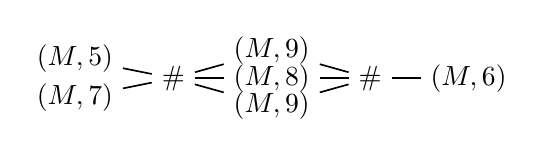
\begin{tikzpicture}[-, >=to, auto, node distance=1.25cm, semithick, transform shape]
\node (M1) {};
\node (T1) [above of=M1, node distance=0.25cm] {$(\tg M,5)$};
\node (B1) [below of=M1, node distance=0.25cm] {$(\tg M,7)$};
\node (M2) [right of=M1] {$\tg\#$};
\node (M3) [right of=M2] {$(\tg M,8)$};
\node (T3) [above of=M3, node distance=0.35cm] {$(\tg M,9)$};
\node (B3) [below of=M3, node distance=0.35cm] {$(\tg M,9)$};
\node (M4) [right of=M3] {$\tg\#$};
\node (M5) [right of=M4] {$(\tg M,6)$};
%
\path (T1) edge (M2);
\path (B1) edge (M2);
\path (M2) edge (T3);
\path (M2) edge (M3);
\path (M2) edge (B3);
\path (T3) edge (M4);
\path (M3) edge (M4);
\path (B3) edge (M4);
\path (M4) edge (M5);
\end{tikzpicture}
}%
\vspace{-1ex}
\newline
where a line from left to right indicates that the item on the right must occur after the item on the left. The end-of-second markers $\tg\#$ separate multisets of natural numbers. So, the set of data traces of $X$ has an isomorphic representation as the set $\Bag(\Nat)^+$ of nonempty sequences of multisets of natural numbers. In particular, the empty sequence $\epsilon$ is represented as $\emptyset$ and the single-element sequence $\tg\#$ is represented as $\emptyset \; \emptyset$.
\end{example}

% A singleton tag alphabet can be used to model sequences or multisets over a basic type of values. For the data type given by $\Sigma = \{\sigma\}$ and $T_\sigma = T$ there are two possible dependence relations for $\Sigma$, namely $\emptyset$ and $\{(\sigma,\sigma)\}$. The data traces of $(\Sigma,T,\emptyset)$ are multisets over $T$, which we denote as $\Bag(T)$, and the data traces of $(\Sigma,T,\{(\sigma,\sigma)\})$ are sequences over $T$.

\begin{example}[Multiple Input/Output Channels]
\label{45:ex:channels}
Suppose we want to model a streaming system with multiple independent input and output channels, where the items within each channel are linearly ordered but the channels are completely independent. This is the setting of (acyclic) \emph{Kahn Process Networks} ~\cite{gilles1974semantics} and the more restricted synchronous dataflow models \cite{lee1987synchronous, benveniste2003synchronous}. We introduce tags $\Sigma_\tg{I} = \{ \tg{I}_1, \ldots, \tg{I}_m \}$ for $m$ input channels, and tags $\Sigma_\tg{O} = \{ \tg{O}_1, \ldots, \tg{O}_n \}$ for $n$ output channels.
The dependence relation for the input consists of all pairs $(\tg{I}_i,\tg{I}_i)$ with $i = 1, \ldots, m$. This means that for all indexes $i \neq j$ the tags $\tg{I}_i$ and $\tg{I}_j$ are independent. Similarly, the dependence relation for the output consists of all pairs $(\tg{O}_i,\tg{O}_i)$ with $i = 1, \ldots, n$. Assume that the value types associated with the input tags are $T_1$, \ldots, $T_m$, and the value types associated with the output tags are $U_1$, \ldots, $U_n$. The sets of input and output data traces are (up to a bijection) $T^*_1 \times \cdots \times T^*_m$ and $U^*_1 \times \cdots \times U^*_m$ respectively.
\end{example}

\section{More Propositions}

\begin{proposition}
\label{45:prop:schema-relaxation-flattening}
If $t: \ss$ and $\ss' \lesssim \ss$,
then there exists a unique $t': \ss'$ such that
every flattening of $t$ is a flattening of $t'$.
\end{proposition}

\begin{proposition}
\label{45:prop:schema-relaxation-decidable}
Schema relaxation, that is on two input schemas $\ss_1$ and $\ss_2$, checking if $\ss_1 \lesssim \ss_2$, and consequently checking schema equivalence, is decidable in quadratic time.
\end{proposition}

% TODO incorporate ALL of this

\subsection*{Proof of Proposition~\ref{45:prop:sps-sequence-correspondence}}

By induction on $\ss$.
For $\relleaf{\mathcal{H}}$,
all three conditions follow by the correspondence between a multiset of items and its linearizations.
%For $\seqleaf{\mathcal{H}}$, (1)-(3) follow since the flattening is unique and $\equiv_{\ss}$ is identity on sequences.
For $\parcomp{\ss_1}{\ss_2}$
and for $\keyby{K}{\ss_1}$,
we observe that sequences over tuples of $\headers(\ss)$ are interleavings of events each from a subschema,
and all such interleavings are equivalent with respect to $\equiv_{\ss}$;
conversely $\equiv_{\ss}$ only holds between different interleavings of the same two or more sequences up to equivalence, i.e. for parallel composition, if $s \equiv_{\ss} s'$ and $s$ is an interleaving of $s_1$ and $s_2$ and $s_1'$ is an interleaving of $s_2'$, then $s_1 \equiv_{\ss_1} s_1'$ and $s_2 \equiv_{\ss_2} s_2'$.
The most interesting case is $\hier{\mathcal{H}}{\ss_1}$.
Here, we essentially apply the idea that $(a \cup b)^{*} = (a^{*} b)^{*} a^{*}$ for languages: in this context $a$ is tuples of $\headers(\ss')$ and $b$ is tuples of $\mathcal{H}$.
So sequences over  tuples of $\headers(\ss)$ decompose into a sequence of subsequences over $\ss'$ delineated by $\mathcal{H}$ events, where there is one more subsequence than the number of $\mathcal{H}$ events.
Since $\mathcal{H}$ events are fully dependent on everything else, this decomposition is not changed by $\equiv$, which can thus be identified with equality on the sequence of $\mathcal{H}$ events together with equivalence on each $\headers(\ss')$ substream.
The definition of flattening reflects this decomposition exactly.

\subsection*{Proof of Proposition~\ref{45:prop:schema-relaxation-flattening}}

We first show uniqueness. Let $t_1', t_2': \ss'$
such that every flattening of $t$ is a flattening of $t_1'$ and of $t_2'$.
Since every SPS has at least one flattening,
we can choose some particular flattening $s$ of $t$
(a sequence over $\headers(\ss)$).
By uniqueness in Proposition~\ref{45:prop:sps-sequence-correspondence}-(1),
since $s$ is a flattening of both $t_1'$ and $t_2'$, $t_1' = t_2'$.

Now we show existence.
As before, choose a particular flattening $s$ of $t$.
Since $\headers(\ss') \supseteq \headers(\ss)$,
$s$ is also a sequence over $\headers(\ss')$.
Thus by Proposition~\ref{45:prop:sps-sequence-correspondence}-(1),
there exists a $t': \ss'$ such that $s$ is a flattening
of $s$.
It remains to show that all flattenings of $t$ are flattenings of $t'$.
Given any flattening $\hat{s}$ of $t$,
by Proposition~\ref{45:prop:sps-sequence-correspondence}-(2b),
$s \equiv_{D_{\ss}} \hat{s}$.
By the definition of relaxation,
$s \equiv_{D_{\ss'}} \hat{s}$.
Then by Proposition~\ref{45:prop:sps-sequence-correspondence}-(2a),
$\hat{s}$ is a flattening of $t'$.

\subsection*{Proof of Proposition~\ref{45:prop:schema-relaxation-decidable}}

We may ignore the headers in $\ss_1$ and not in $\ss_2$.
Then for each pair of headers $H, H'$ in $\headers(\ss_2)$,
we build a formula $\phi^1_{H, H'}$ whose free variables are the fields
in $H$ and the fields in $H'$,
which describes when
$x D_{\ss_1} x'$ for $x : H$ and $x' : H'$.
This is done by expanding out Definition~\ref{45:def:dep-relation}.
In all case the formula built is either true or false, or derived
from a subcase,
except in the $\keyby{K}{S}$ (and bag) cases where
$\tuprestrict{x}{K} = \tuprestrict{x'}{K}$ arises as an atomic
formula.
Altogether, each $\phi^1_{H, H'}$ is just an atomic formula over the
language of equality.
We do the same for $\ss_2$ to get formulas $\phi^2_{H, H'}$.
The problem now becomes checking a set of implications
of atomic formulas over the language of equality, which is
decidable by checking each implication
$\phi^1_{H, H'} \to \phi^2_{H, H'}$
in turn
and inspecting the variables $\tau_i$ where $\tau_i$ is
a type present in an attribute $\hdrfield{\alpha_i}{\tau_i}$ of $H$ or $H'$.
The complexity is quadratic because there are quadratically many pairs $H, H'$.
% deciding the formula amounts to enumerating whether the number of elements in $H$
% is at least some fixed finite number.

\section{Discussion}

\subsection{Other language constructs}

Singleton and Relation

% We also have the following abbreviations:
% \[
%   \relleaf{T} := \keyby{T}{\singleton{\unittype{}}}
% \]
% where $\unittype{}$ denotes the unit type, and

% \inference[Singleton]
% {
%   t: T
% }
% {
%   \batchtype{t}{\singleton{T}}
% }
% \inference[Singleton]
% {
%   e: T
% }
% {
%   \eventtype{e}{\singleton{T}}
% }
% \inference[Singleton]
% {
%   t: T
% }
% {
%   \lintype{[t]}{\singleton{T}}
% }

\subsection{Incrementality}

Batches and linearizations represent static views of an entire stream, bundled up as one object.
One thing missing from the presentation in this section is an incremental view of streams.
For example, one idea of a way to define a stream incrementally is via a generator object which produces events of the stream:
\[
\inference[Generator]
{
  \texttt{State}: \texttt{Type} \\
  f: \texttt{State} \to \texttt{Option<}\texttt{Event}(S) \times \texttt{State>}
}
{
  \texttt{Generator}(f): S
}
\]

Composing these generators, though, requires care as they must be consistent with the types. An event-by-event view of stream operators is discussed more in \Cref{cha:distribution} and what it means for these operators to be consistent with the stream types and parallelizable.

% \section{Historical Notes}
% TODO
